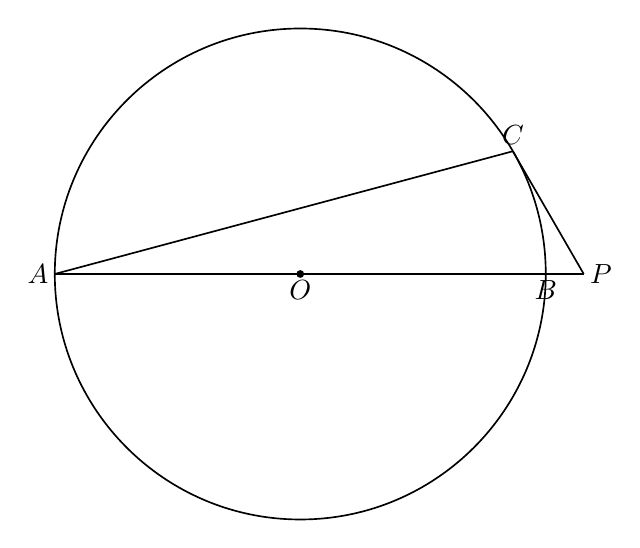
\begin{tikzpicture}[x=1cm,y=1cm,line width=.6pt,font=\normalsize]
\coordinate (O) at (0,0);
\coordinate (A) at (-3.11769145,0);
\coordinate (B) at (3.11769145,0);
\coordinate (C) at (2.7,1.55884573);
\coordinate (P) at (3.6,0);
\draw (O) circle[radius=3.11769145cm];
\draw (A)--(P);
\draw (A)--(C);
\draw (C)--(P);
\node[left=2pt,inner sep=0pt] at (A) {$A$};
\node[below=2pt,inner sep=0pt] at (O) {$O$};
\node[below=2pt,inner sep=0pt] at (B) {$B$};
\node[above=2pt,inner sep=0pt] at (C) {$C$};
\node[right=2pt,inner sep=0pt] at (P) {$P$};

% Explicit named circle-center points, painted after all region fills.
\fill (O) circle[radius=1.4pt];
\end{tikzpicture}
